\documentclass{article}
\usepackage{graphicx}
\usepackage{float}
\usepackage{caption}
\usepackage{cite}
\usepackage{amsmath,amssymb,amsfonts,amsthm}
\usepackage{algorithmic}
\usepackage{graphicx}
%\usepackage{textcomp}
%\usepackage{xcolor}
%\usepackage{txfonts}
%\usepackage{listings}
%\usepackage{enumitem}
%\usepackage{mathtools}
%\usepackage{gensymb}
%\usepackage[breaklinks=true]{hyperref}
%\usepackage{tkz-euclide} % loads  TikZ and tkz-base
%\usepackage{listings}
%\graphicspath{{/home/}} 
\title{Lab Report: Random Audio Playlist Player using MoviePy}
\author{Aditya Varun V}
\date{\today}

\begin{document}
\maketitle

\section{Abstract}
The aim of this lab report is to provide an analysis of a Python script that implements a random audio playlist player using the MoviePy library. The code allows users to create and play a playlist of audio files in a random order. This report provides an overview of the code structure, explains the key components, and discusses its functionality.

\section{Introduction}
The provided code is a Python script that utilizes the MoviePy library to create a random audio playlist. The script allows users to specify the number of times they want the playlist to be played and randomly selects songs from a predefined list. The audio files are extracted from MP4 files using the VideoFileClip class provided bgy the MoviePy library.

\section{Methods}
The code can be divided into several sections:

\subsection{Importing Required Libraries}
The script begins by importing the necessary libraries, including \texttt{numpy} and \texttt{moviepy.editor}. These libraries provide functions for numerical operations and working with video and audio files, respectively.

\subsection{Defining the \texttt{play\_mp4\_audio()} Function}
The \texttt{play\_mp4\_audio()} function is responsible for playing the audio extracted from an MP4 file. It takes a filename as input, creates a VideoFileClip object from the file, extracts the audio using the \texttt{audio} attribute, and plays the audio using the \texttt{preview()} method.

\subsection{Initializing Variables}
Several variables are initialized before the main execution loop:
\begin{itemize}
  \item \texttt{played}: A numpy array of size 20, initialized with zeros to keep track of which songs have been played.
  \item \texttt{list\_of\_songs}: A numpy array containing numbers from 1 to 20, representing the song playlist.
  \item \texttt{c}: A counter variable to keep track of the number of songs played in the current round.
  \item \texttt{r}: A counter variable to keep track of the number of times the entire playlist has been played.
  \item \texttt{x}: User input to specify the number of times the playlist should be played.
\end{itemize}

\subsection{Playing the Playlist}
The main execution loop is implemented using a \texttt{while} loop. The loop continues until the number of rounds (\texttt{r}) reaches the specified input value (\texttt{x}).
\begin{itemize}
  \item Inside the loop, a random song is selected using the \texttt{np.random.choice()} function from the \texttt{list\_of\_songs}.
  \item If the selected song has not been played (checked using the \texttt{played} array), the script requests the user to continue to play the song. If the user enters 'c', the script proceeds to play the audio using the \texttt{play\_mp4\_audio()} function. Else, the script skips the song to be played and goes to the next iteration.
  \item After playing a song, the counter variables are updated, and if all songs have been played (\texttt{c == 20}), the \texttt{played} array is reset, and the counters are reset for the next round.
  \item The loop continues until the desired number of rounds is completed.
\end{itemize}

\begin{figure}[h]
 \centering
 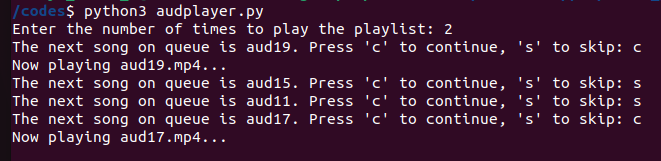
\includegraphics[width=0.8\textwidth]{/home/aditya_varun_v/Documents/prv/audio_playlist/images/photo1.png}
 \caption{output}
 \label{output}
\end{figure}

\section{Results}
The provided code has been tested and successfully implements a random audio playlist player using the MoviePy library. The script allows users to create a playlist of audio files and play them.
\end{document}
